\documentclass[conference]{IEEEtran}
\IEEEoverridecommandlockouts
% The preceding line is only needed to identify funding in the first footnote. If that is unneeded, please comment it out.
\usepackage{cite}
\usepackage{amsmath,amssymb,amsfonts}
\usepackage{algorithmic}
\usepackage{graphicx}
\usepackage{textcomp}
\usepackage{xcolor}
\usepackage{listings}
\def\BibTeX{{\rm B\kern-.05em{\sc i\kern-.025em b}\kern-.08em
    T\kern-.1667em\lower.7ex\hbox{E}\kern-.125emX}}
\begin{document}

\title{SeL4 verfication in Isabelle/HOL and \\
verification of a OpenBSD driver}

\author{\IEEEauthorblockN{Adriana Stancu}
\IEEEauthorblockA{\textit{University of Bucharest}\\
Bucharest, Romania  \\
adriana.stancu@unibuc.ro}
\and
\IEEEauthorblockN{prof. dr. Ioana Leustean}
\IEEEauthorblockA{\textit{University of Bucharest}\\
Bucharest, Romania \\
ioana@fmi.unibuc.ro}
\and
\IEEEauthorblockN{conf. dr. Paul Irofti}
\IEEEauthorblockA{\textit{University of Bucharest}\\
Bucharest, Romania  \\
paul.irofti@unibuc.ro}
}

\maketitle

\begin{abstract}
The seL4 microkernel is currently the only kernel that has been fully formally verified. In general, the increased interest in ensuring the security of a kernel\textquotesingle s code results from its important role in the entire operating system. \\
One of the basic features of an operating system is that it abstracts the handling of devices. This abstraction is represented by device drivers - the software that manages the hardware. A proper verification of the software component could ensure that the device would work properly unless there is a hardware failure. \\
This is the motivation why we choose to try to model the behavior of a device driver and build the proof that the code implementation matches the expected behavior. The proof was written in Isabelle/HOL, the code translation from C to Isabelle was done automatically by the use of C-to-Isabelle Parser and AutoCorres tools. We choose Isabelle theorem prover because it’s efficiency was already shown by being used through the verification of seL4 microkernel.
\end{abstract}

\begin{IEEEkeywords}
Isabelle, C programming language, verification, kernel, driver
\end{IEEEkeywords}

\section{Introduction}
The kernel is a crucial component of a system, and direct access to hardware resources leads to an increased risk if a malfunction occurs. In our case, seL4 was designed as a microkernel in order to reduce the impact of software problems to the system\textquotesingle s functionalities.\\
The main topic of interest in the analysis of the seL4 microkernel is the way to prove the functional correctness through the Isabelle/HOL theorem prover. The methods applied in system verification are more powerful and accurate than automated verification techniques such as model checking, static analysis, or deploying the entire kernel in a type-safe language. \\
This method of proving in Isabelle all the critical properties of the systems allows the analysis of specific aspects such as exploring the branches of execution of safe scenarios (safe execution), but also a set of specifications and proofs of kernel behavior reaching the analysis of implementation in C of the kernel for the ARM platform.
\section{SeL4 verification structure}
Although work to implement its proofs was started in 2009 \cite{sel4} by the National ICT Australia - NICTA (Information and Communication Technology Research Center) research team, formal proofs of the kernel are still maintained up to date with the source code.\\
SeL4 is part of the L4 family - along with other implementations that share the same L4 interface: Pistachio \cite{pistachio}, Fiasco \cite{fiasco} or Hazelnut \cite{hazelnut}.\\
The proofs that underlie the verification of seL4 system are in the form of Hoare structures that have in their center a code component or whole functions. The difficulty of verifying the seL4 micro-kernel lies in formulating pre-conditions and post-conditions that accurately represent security properties that it must meet. At the same time, the formal representation must be as close as possible to the structure and functionalities implemented in the source code.\\
An interesting aspect related to the design of a microkernel and the properties of the C code in relation to the form of their verification is the separation of calls to kernel functions in two phases \cite{verifos}: verification and execution. The verification phase can be understood as a stage of validation of the preconditions: the input data and the permissions on the actions to be performed are verified. The execution consists in the actual running of the system function, benefiting from its verification because the preconditions have already been verified in the previous phase. \\
An important thing to note is that in the verification phase, the status of the system is not changed, otherwise this separation would no longer be relevant. And the idea brings a valuable advantage in the verification process because it simplifies the system call proof: execution will not return an error if the verification phase has been completed successfully.
\section{SeL4 memory management}
The seL4 kernel uses a memory allocation model that transfers the control over the allocation of memory from kernel space to applications that have this permission. Permission on memory management is represented by having a structure called capability \cite{sel4-wp}.\\
A consequence of this transfer of rights is that the kernel heap memory can be precisely partitioned between applications: each application has that part of the heap for which it has a capability that gives it that authority. Separating heap memory is especially important for expressing and demonstrating security properties (integrity and confidentiality).\\
The basic features of the kernel memory allocation model are as follows \cite{verifos}:
\begin{itemize}
    \item Memory allocation is explicit and is performed only when assigning a type (retype) to an untyped memory area.
    \item The memory allocation is strictly delimited by the specified free memory.
    \item Kernel objects are not shared or reused.
\end{itemize}
This memory management model leaves the responsibility for verifying security policies outside the kernel. All that is left is to verify the correctness of the memory allocation algorithm in the kernel. The properties of interest being:
\begin{itemize}
    \item Checking that the allocated objects are contained in the corresponding areas of free memory;
    \item Memory areas allocated to objects do not overlap.
\end{itemize}
As specified, the rights for allocating a certain memory area are represented by holding a capability, these capabilities can be transferred between the kernel components, their transfer can be represented in the form of a tree in which the capabilities are the nodes of the tree.\\
If for the memory allocation the two properties listed above must be checked, which ensures the separation from the rest of the objects and the integrity of the newly assigned object, for its dislocation two steps are applied to invalidate all references to the memory area to be dislocated:
\begin{enumerate}
    \item Searching for all the capabilities by which access rights are granted on the memory object;
    \item Delete all these capabilities and mark the memory area as free (return it to the unallocated memory block).
\end{enumerate}
For the first stage, the capability transfer tree is used to find and invalidate all capabilities that allow permissions on the memory area. In the second stage, it is verified through the same tree that there are no references in other objects or global references to the area to be released.
\section{Memory access verification}
Memory access is an interesting topic in order to model as accurately as possible the behavior of program C. In Isabelle, pointers can be represented as a new type of data in the form: datatype a ptr = Ptr word32, which means that a pointer can be represented only by the word32 address it contains. Using this representation one can reason about the heap memory.\\
In this sense an important problem is raised by the cases in which it is possible to pass from one type of pointer to another. For example, if we have two different pointers as type (float and int), after we change the value from the address to which one of them points, we cannot be sure that the other has not been changed, if they would have indicated from the beginning to the same address. To ensure that different pointers as a type point to different addresses, the Burstall-Bornat model was used as a solution \cite{burstall}.\\
The solution developed by Burstall and Bornat is to use a model in which the heap memory is separated into types. Each data type has its own function that maps pointers to their values:\\
record state =\\
  heap\_int ∶∶ word32 $ \Rightarrow $ int\\
  heap\_float ∶∶ word32 $ \Rightarrow $ float\\
  heap\_intptr ∶∶ word32 $ \Rightarrow $ addr...\\
This model avoids ambiguities when a pointer of a certain type is modified. In the previous example, if we changed the values contained in the address of an integer pointer, there is no confusion that a pointer to a float value was accidentally changed because the values of the float type are separated from each other. Of course, the fact that this model gives us the certainty that we do not accidentally change values of different types, however, also brings the limitation that it is no longer possible to switch from one data type to another by cast. A memory area, once allocated, remains defined in the corresponding heap memory section until it is released.
\section{C to Isabelle conversion}
The most interesting component of the formal check in seL4 is the bridge between C language and the proofs in Isabelle. This is also the most complex part of the proofs because the semantics of the C language must be taken into account, memory management including data types, storage of structures in memory, pointer cast between different data structures or pointer arithmetic. \\
For example, in Isabelle, memory addressing is represented by a function defined on the address space resulting in binary data, without information about the type of data to which the address refers. Apart from this function that models pointers, the way different types of data are stored is treated separately. \cite{tuch} Abstracting how memory access, data alignment, and how different data types are modeled helped that higher-level proofs not require repetitive checks, such as that a pointer is not null before being accessed, because these checks are already defined as constraints.\\
The correctness of the C language semantics is not, however, treated as critical to the proofs of the whole system because it adds an additional level to the verification: the validation of the correspondence between the formal model and the result obtained after compiling the source code. However, this validation brings the expected results when the code is compiled with a low level of optimizations. Therefore, the exclusive use of checking the resulting binary file without taking into account the source code was not completely performed.\\
The proof technique used to ensure the correspondence between the abstract specifications, the formal model of the source code and the model resulting from the analysis of the binary file is the refinement. "Program C is a refinement of program A, if the set of behaviors of program C is a subset of the behaviors described by program A" \cite{verifos}. Behavior means a sequence of steps given by the change of system state and the transition between states. The state of the system consists of the state of its components (memory, processes, resources) both those belonging to the user space and those in the kernel.
\subsection{Isabelle/HOL theorem prover}
Isabelle is an interactive theorem prover that supports several types of formal logic systems. Isabelle/HOL is Isabelle\textquotesingle s specialization of Higher Order Logic (HOL). HOL is a type-based logic whose system resembles the one from functional programming languages \cite{funcprog}. Existing types can be classified \cite{sel4} into:
\begin{itemize}
    \item basic types, for example the bool(boolean), nat($\mathbb{N}$) or int($\mathbb{Z}$);
    \item type constructors, for example list and set types. Type constructors are written postfix, that is, after their arguments. For example, nat list is the type of lists whose elements are natural numbers.
    \item types of functions are denoted by "$\Rightarrow$";
    \item types of variables are denoted by $'a, 'b$, etc.
\end{itemize}
Terms are represented as in functional programming by applying functions to certain types of arguments. If we have $f$ a function of type $\tau_1 \Rightarrow \tau_2$ and $t$ is a term of type $\tau_1$ then $f t$ is a term of type $\tau_2$. In Isabelle the notation $t::\tau$ is used to represent that the term $t$ is of type $\tau$.
Isabelle\textquotesingle s proofs are structured in theories. A theory is a collection of types, functions and theorems, just like a module in a programming language. A theory has the following format:
\begin{lstlisting}
theory T
imports B1 ... Bn
begin
statements, definitions, proofs
end
\end{lstlisting}
Where B1 ... Bn are the names of the existing theories on which the T theory is based. Each T theory must be in a file called T.thy. HOL contains a Main theory, which contains all predefined basic theories, such as arithmetic, lists, or sets. A theory can include a list of more .thy file, this way we only have to include  "AutoCorres.AutoCorres" to have all theories needed for parsing and basic proofs.\\
The proofs can have the form of theorems or lemmas, both can be used inside other proofs. There are some keywords for applying them in order to reach some goal \cite{isabelle}, for example the most common keywords used in our proofs are: \textit{unfolding x} - which applies the definition of \textit{x} on the current goal and \textit{apply x} - which refers to other theorems or set of rules to be used.

\subsection{Parsing C to Isabelle}
Approaching the C language from the perspective of obtaining a semantic model on which valid reasoning can then be built is an important contribution of the seL4 system and deserves to be studied in detail. Several steps were taken to translate the C code from seL4 into Isabelle \cite{greenaway}:
\begin{enumerate}
    \item Each C source file is parsed by an external C preprocessor, which extends "\#include" formulas and macro commands as well as other preprocessing directives;
    \item The resulting C file is then translated into Simpl by the C-to-Isabelle analyzer \cite{tuch} developed by M. Norrish, H. Tuch and G. Klein;
    \item Each structure used in the program is represented by a record in Isabelle;
    \item Local and global variables are analyzed to generate two new types: a record called globals, which contains information about global variables, and \textit{"a myvars"} record for local variables;
    \item Each individual function is translated into its equivalent representation in Simple language;
    \item Demonstrations are performed on the generated functions, to specify which global variables modify the function.
\end{enumerate}
The post-translation steps in Simpl are embedded in the AutoCorres tool developed by D. Greenaway and specified in detail in his doctoral dissertation \cite{greenaway}. Because this tool uses the result of the C-to-Isabelle parser as input, AutoCorres supports the same subset of the C language. Programs that support loops, function calls, cast between various types, pointer arithmetic, structures, and recursion are supported. On the other hand, as described in the verification of the seL4 system in general, the following are not supported: references to local variables, expressions "goto" or "switch", unions, arithmetic operations in floating point or the use of pointers to functions. \\
In his paper \cite{greenaway}, D. Greenaway describes using the illustrative example shown below, how one can go from the implementation in C of a simple function to the result of the C-to-Isabelle parser - with which it is quite difficult to work, and then to the final form that will be reached after running the AutoCorres tool on the result.\\
In essence, the purpose of the AutoCorres tool is to abstract the low-level representation given by the C-to-Isabelle parser into a high-level one by the following:
\begin{itemize} 
    \item performing the conversion between the deeply embedded representation (as will be described below) and the shallowly embedded one;
    \item abstraction of arithmetic operations at machine word level (represented on 32 bits) in operations on the whole set of integers and natural numbers;
    \item abstracting the heap memory at byte level in separate areas depending on the data type using the Burstall-Bornat model \cite{burstall};
    \item simplifying the code and translating the type of variables from the representation into Simple into a form that is easy to reason in Isabelle.
\end{itemize}
\textbf{Deeply vs shalowly embedded representations.} Before we can begin to formally reason about a program, we must first translate it into the logic used by our theorem demonstrator. To bring the C code into Isabelle, it was necessary to decide which aspects of the code would be translated into the demonstrator logic. If the emphasis is on the structure of program C and its preservation in Isabelle, we say that deeply embedded representation was used, and if the semantics of the program are important in the translation process, then we have a shallowly embedded representation of the source code in Isabelle logic. AutoCorres has as its role the conversion between the structural representation of the C language given by the C-to-Isabelle parser in the semantic representation on which reasoning can then be performed.\\
An illustrative example used by Greenaway \cite{greenaway} to explain the difference between the two forms of code representation is given by the observation on the following equation: 2 + 2 = 4. If we want to prove that the left side is equal to the right one, we can perform the addition (treating the expression as shallowly embedded) and state that the sentence is true. But if we look at the structure of the equation (deeply embedded), on the left we have 3 characters and on the right only one. So we can say that the two parts are not equal because we did not give any semantics to the assembly operation and its terms. Structural treatment is not helpful if we want to prove certain statements about a program. For this reason, the semantic representation of the C code is an important contribution in the verification of the seL4 kernel, and this is done through the Greenaway\textquotesingle s AutoCorres tool.\\
The semantic representation obtained with AutoCorres aims to capture the behavior of C programs, the representation in Isabelle that the program can change the overall state of the system, can contain loops for which there is a possibility that they may not end, may have exceptions or other errors and it can treat them differently or it can contain random choices. Many of these requirements are covered by the extensive use of existing monads in Simpl (Skip, Basic, Cond, Guard, etc.) and the addition of new constructions such as: gets, return, whileLoop. The latter brings the greatest similarity between the source imperative language and the functional one in which it is modeled.
\subsection{C subset limitations}
Of course, C-language constraints were required, so we are using only a subset of the C99 standard specifications \cite{iso}. One of the most relevant restrictions is that pointers to functions are not supported. Pointer data types are defined as functions that must return data stored at those addresses. In this case, if the pointers refer to the address of a function, there is no guarantee that the reference cannot be circular, and the address of the function must also be resolved. \\
Also, sequences that could change the flow of the code, such as code jumps using "goto" or "switch", are not supported. Other components that are not supported due to the unpredictability of the GCC compiler when it might try to optimize the positioning of data in memory are unions or bit fields.\\
\subsection{Limitation case - calling function pointers}
The limitation of not being able to call functions that were set via their address to a function pointer was a major drawback in the integration of the driver because we need to address programable tasks to be executed in the future. The tasks may come from the device driver, the timer or other additional file but the main loop should only the the corresponding function that was set via its pointer. A simplified program would be the one below where the C-to-Isabelle parser fails to translate the last function because the call to \textit{foo()} is done via the function pointer \textit{p\_fun}. 
\begin{lstlisting}[language=C]
static int counter;

void foo(void) { counter++; }

void (*p_fun)(void);

void set_function(void) { p_fun = foo; }

void call_function(void) {
    if(p_fun) p_fun();
}
\end{lstlisting}
Currently, there are a few workarounds valid for this situation, but all of them cannot provide the full proof, they only skip certains parts of the program or proofs in order to provide a translation avoinding the part were the function pointer is used:
\begin{itemize}
    \item skip parsing the \textit{call\_function} by adding the \textit{/** DONT\_TRANSLATE */} adnotation, this variant was used during the proof because the other translations ar enot affected, we only had to avoid proving some properties that involved the function pointer;
    \item add the following adnotations before parsing the C file, this will assert those theorems as axioms rather than try to prove them:
\begin{lstlisting}
declare [[quick_and_dirty = true]]
declare [[sorry_modifies_proofs = true]]
\end{lstlisting}
    \item add some other adnotations before parsing the C file, this will not try to prove the theorem involded in function pointers:
\begin{lstlisting}
[[calculate_modifies_proofs = false]]
\end{lstlisting}
\end{itemize}
\section{Driver verification}
Drivers are pieces of software part of monolithic kernel (but can also run is userspace), whose purpose is to interact with hardware devices or buses and to provide a interface between the kernel and those components. We choose to verify drivers as a further development of seL4 verification because the drivers are independent enough from the kernel structure, thus the verification process does not need to take into consideration the particularities of the kernel where the driver came from. \\
The main objective of driver modeling in Isabelle is to generalize the verification of kernel drivers. We started from an OpenBSD driver which was adapted to only use basic C function instead of kernel depended ones. This simulation comes at a cost, we have to assume that the rest of the system works correctly because the verification will cover only the driver functionalities. \\
The parts for which we applied this assumption are the hardware related components like bus communication and reading/writing form device registers. We suppose that the bus works correctly and the register behavior matches the datasheet specifications. In general cases, this separation between the software driver and the hardware components is helpful to investigate if some strange device behavior is generated by a hardware fault or the software does not work as expected.

\subsection{OpenBSD octrng driver}
The driver used for prototyping seL4 verification is a hardware random number generator for Octeon boards \cite{octrng}. We choose this driver because it has a small configuration sequence and it is pretty isolated from the OpenBSD kernel (there are no major dependencies from other drivers or kernel components). The driver structure is very simple, it has two important functions:
\begin{itemize}
    \item \textit{octrng\_attach} - driver initialization routine, its purpose is to configure the hardware in order to start generating random values. It maps the registers of the device in local address space and sets bits 62 and 63 (OCTRNG\_ENABLE\_OUTPUT, OCTRNG\_ENABLE\_ENTROPY) from the register 0x1180040000000 (OCTRNG\_CONTROL\_ADDR). By setting the output and entropy flags, the device will start generating random values. The output is then read every 10 miliseconds.
    \item \textit{octrng\_rnd} - a periodic call of this routine will provide each time the result from the device. The random value is retrieved from the register 0x1400000000000 (OCTEON\_RNG\_BASE + OCTRNG\_ENTROPY\_REG). This value will be added then to the entropy pool each time this function is called.
\end{itemize}

\subsection{Sample driver for verification}
Before parsing the C driver implementation into Isabelle, some kernel particularities had to be implemented separately because we extracted only the driver file, not the other kernel functionalities included by the headers. We only had four components that had to be mimicked in new functions or files in order to fulfill the octrng driver interactions:\\
\textbf{Bus communication.} In the original driver, the bus is accessed via \textit{bus\_space\_x()} functions, where \textit{x} can refer to register mapping, reading or writing on the bus. In our case, we replace the buss access with simple reading or writing to local memory. This way, the bus is supposed to always deliver the read/write commands except the timing (a bus write may need more time than writing to a local variable). But in this case the timing is not relevant because all actions are done sequentially.\\
\textbf{Device registers.} Because the bus communication is removed, we had to find a way to express the register behaviour using local memory. So the implementation separated the useful registers in a static structure. For octrng driver, we only need the control register, so we have the structure \textit{rng\_regs} with only one member \textit{control\_addr} which will be the absolute address of the control register.
\begin{lstlisting}[language=C]
static struct reg {
  unsigned long control_addr;
} rng_regs;
\end{lstlisting}
Reading or writing the device’s register is usually done by mapping the physical registers in memory. Usually this involves a communication with the device via the bus on which it is located. For our model however, the device is just a representation of the actual one, so there are no physical registers and our transfers on the bus are simply reading or writing operations from the device register structure. \\
There is a important point for our model resemble as much as possible the real one: the internal register behaviour. In our case, only some registers are important and we have to cover these cases: enabling the output bit, the entropy bit and reading the control value. These cases are implemented inside two functions \textit{set\_register} and \textit{get\_register}. The first function modifies the required register with a given value while the second one reads a register or returns the value of the current timer if both output and entropy flags are set. \\
\textbf{Global timer.} The timer has two functions thorough the driver implementation. One is inherited from the original driver: scheduling the random function to be repeated every 10 milliseconds. The other has been added for verification purposes while the actual hardware device is missing: mimicking the random value by returning the timer value instead of the random value from the device register. Because we do not have access to an actual timer either, we will simply use a global variable that will be incremented by the \textit{idle()} function each time the main loop chooses a task to be scheduled.\\
\textbf{Task scheduling.} The initialization call to the \textit{attach} function of the driver is done from a separate file that has the purpose to simulate a very simple scheduling of tasks. Basically, this is a loop guarded by a timeout, and we check for tasks waiting to be scheduled during each iteration. This loop also calls the \textit{idle} function to increase the global timer. The tasks are stored into a static array of tasks, each task having the following components:
\begin{lstlisting}[language=C]
typedef struct {
    int timeout;
    unsigned long start;
    void (*timeout_fun)(void);
} Task;
\end{lstlisting}
Scheduling a task to run some \textit{foo()} function after 3 time units in the future means to call the function that sets a new task in the task queue with \textit{timeout} set to 3, \textit{start} set to current time value and \textit{timeout\_fun} pointing to the \textit{foo()} function. The task queue is a circular buffer, each task addition increments the index of the newest task added. After finnishing a task, it will be erased from the array. 

\subsection{Proving driver function correctness in Isabelle}
Our driver representation is translated into Isabelle/HOL by applying successively the C-to-Isabelle parser and then the AutoCorres tool. A limitation of these tools is that we can only parse one .c file at a time and provide one corresponding .thy file. In seL4, some of the .c files have produced isolated theory files and these theories are then included where needed. However, there is a starting point to parse all the other files and this is the \textit{kernel\_C} preprocessor output file. We used the same approach by including the \textit{octrng} driver and the timer implementation inside the .c file containing the main loop. This file can be reprocessed by running the command 
$gcc -DINCLUDE\_C\_FILES -E -CC run\_tasks.c > run\_tasks.c\_pp$ and producing the \textit{run\_task.c\_pp} file which will be used as input for the Isabelle translation.\\
The \textit{INCLUDE\_C\_FILES} compilation flag was added in order to easely switch between including the header and .c files into the main loop. The .c files are needed to be included instead of the headers because the otherwise we will not get the translation of the function implemented in the additional .c files. \\
The structure of the theory file contains the import statements that include AutoCorres theories and all the helper theories. The C-to-Isabelle parser is applied by simply declaring the input preprocessed file and calling the \textit{install\_C\_file}. After this step we have all the C function translated into SIMPL theorems. In order to obtain the final representation of those theorems, the AutoCorres tool is applied on the target file. Inside the main context of this theory we can start defining new terms, functions or proving new lemmas about the translated C functions.
\begin{lstlisting}[basicstyle=\small]
theory Run_Tasks
  imports 
    "AutoCorres.AutoCorres" 
begin

external_file "run_tasks.c_pp"
install_C_file "run_tasks.c_pp"
autocorres "run_tasks.c_pp"

context run_tasks begin
definitions, lemmas, theorems ...

end
\end{lstlisting}
After the translation into Isabelle is finished, we can access the functions from C as theorems in Isabelle. For example, a C function \textit{foo} is represented as a theorem named \textit{foo’\_def}. The definition of a function can be viewed in JEdit by typing $thm foo^\prime\_def$. All the additional functions implemented in all the included files will be translated. We will analyze only the two functions related to the \textit{octrng} driver: \textit{octrng\_attach} and \textit{octrng\_rnd}. Also the constants defined in .c file needs to be redefined if we want to use the same names through the new theorems or lemmas. The C constants have been translated directly into their values, but we can give a name to the same values as Isabelle definitions (for example the enable output flag will be defined in Isabelle as \textit{definition} ``OCTRNG\_ENABLE\_OUTPUT $\equiv (1 << 1) :: $ word32``).\\
\textbf{The attach function.} This is where the device configuration takes place and also the task of periodically checking the value is programmed. The Isabelle translation of the function in Fig. 2 matches the C code: the flags of the control register are set accordingly. \\
\begin{figure}[htbp]
\centerline{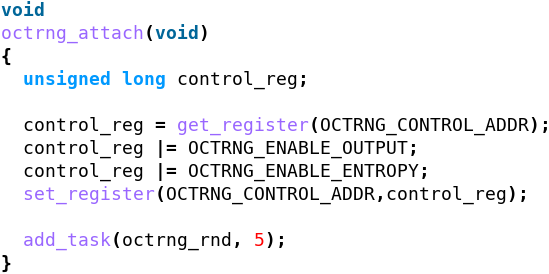
\includegraphics[width=0.4\textwidth]{attach_c.png}}
\caption{\textit{octrng\_attach} C implementation} 
\label{fig}
\end{figure}
\begin{figure}[htbp]
\centerline{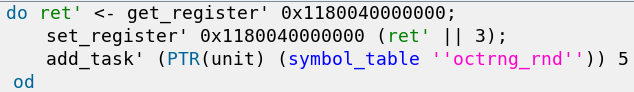
\includegraphics[width=0.45\textwidth]{attach_thy.png}}
\caption{\textit{octrng\_attach} Isabelle definition} 
\label{fig}
\end{figure}
What we would like to verify from this function is that, after the execution of \textit{octrng\_attach} the device state is ready for generating random values, i. e. the control register is set corectly. We can model this inside a lemma in the form of a Hoare triple $\{P\} C \{Q\}$, where $P$ and $Q$ are the precondition and respectively the postcondition, C is the executed program. In our case, we want to verify that running the $octrng\_attach$ program function in any program state, the control register will have set to 1 the flags for enabling output and entropy. So the precondition is always $True$ because there are no requirements and int the postcondition we check the bits of the flags. 
\begin{figure}[htbp]
\centerline{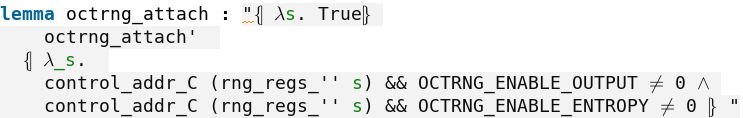
\includegraphics[width=0.45\textwidth]{attach_lemma.png}}
\caption{\textit{octrng\_attach} verification lemma} 
\label{fig}
\end{figure}
This proof is straightforward, we only need to use \textit{unfolding} to apply all the functions and definitions needed. The weakest precondition tool (\textit{wp} command) will compute the necessary precondition that we have to prove further. All the provided goals can be derived automatically from the function definition. Except for the bit operations for which we need to explicitly apply the \textit{word\_bitwise} theorems.

\textbf{The periodic “rng” function.}
This function should constantly retrieve the “random” value and add it to the pool. Because we only have the driver part and not the rest of the OpenBSD kernel, this value will be the timer value and the randomness poll is just a global variable which will be updated by calling this function. The C implementation just reads the value of the output register and saves it into \textit{rand\_value} global variable, then schedule another function execution after 10 time units. The Isabelle representation matches the same behavior, the only thing different here is that all the global variables from the C program are now represented as Isabelle terms, for example the integer \textit{rand\_value} is translated in Isabelle as \textit{rand\_value\_''} a term of type sword32 (signed word on 32 bits).
\begin{figure}[htbp]
\centerline{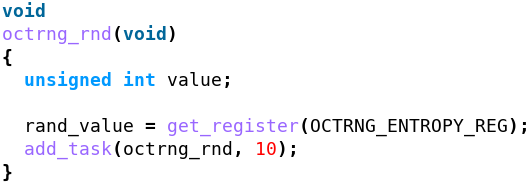
\includegraphics[width=0.38\textwidth]{rnd_c.png}}
\caption{\textit{octrng\_rng} C implementation} 
\label{fig}
\end{figure}
\begin{figure}[htbp]
\centerline{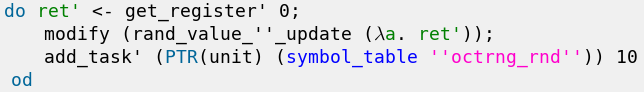
\includegraphics[width=0.45\textwidth]{rnd_thy.png}}
\caption{\textit{octrng\_rng} Isabelle definition} 
\label{fig}
\end{figure}
The verification lemma for \textit{octrng\_rnd} has a few more preconditions than the initialization function because we have to firstly make sure that the function can be executed (the task queue is not full) and then that the driver is configured properly (the output and entropy flags are set). 
\begin{figure}[htbp]
\centerline{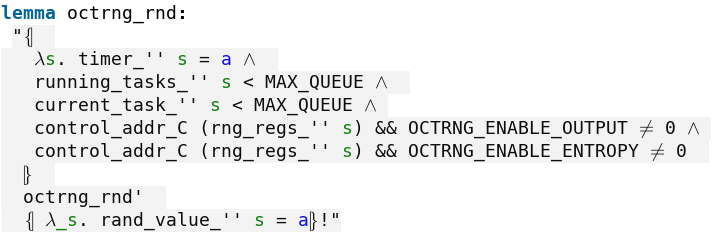
\includegraphics[width=0.45\textwidth]{rnd_lemma.png}}
\caption{\textit{octrng\_rng} verification lemma} 
\label{fig}
\end{figure}
The additional clause $ \lambda s. timer\_’’ s = a$ represents that is any given state $s$ the global timer variable may have a label $a$ for its value. What we want to prove it that the same value will be set to the global \textit{rand\_value} and this is the precondition $ \lambda\_ s. rand\_value\_’’ s = a$. The verification will be done using the same proofs as for the previous lemma: first we apply the definition of all functions used and the apply the weakest precondition tool. The goals obtained this way are easily to prove by applying the auto method.\\
This lemma could be improved by adding some other specifications like checking that the same function will be called after 10 time units or that the function will be always called in time. The proofs that involve task scheduling were avoided because the translation of the funciton that runs the actual task is not parsed as described in the C subset limitation section.\\
\textbf{Main loop and other lemmas.}
The driver functions are bound toghether inside a small program that simulate a simple scheduler of tasks. The main loop does the initialization of the environment including the call of the \textit{octrng\_attach} function, then a main loop will check for each time unit if there are tasks whose timeout expired so their function has to be run. We can add lemmas for those additional functions mainly because some of they might be useful in proving other properties. For example, a simple function \textit{idle} increases the global timer after each iteration of the main loop. The lemma for this function could verify that the timer is modified exactly by 1 after running this function in any program state.
\begin{figure}[htbp]
\centerline{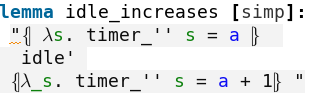
\includegraphics[width=0.25\textwidth]{idle_lemma.png}}
\caption{A lemma for \textit{idle} function} 
\label{fig}
\end{figure}
Its proof is evident, we only have to apply weakest precondition tool and then the \textit{auto} method for applying the simplifications. A proof that is more interesting is the one that states the main loop runs until a timeout occurs. This is done by limiting the timer with a maximum value, if this value is reached no other task will be called. 
\begin{figure}[htbp]
\centerline{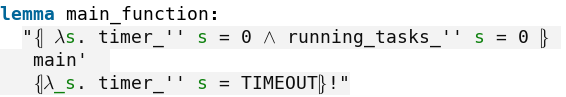
\includegraphics[width=0.4\textwidth]{main_lemma.png}}
\caption{A lemma for \textit{main} function} 
\label{fig}
\end{figure}
The difference between this lemma\textquotesingle s proof and the other is that here we have loops so we have to first provide a proof that those loops ends. Because the function that actually runs the task is not parsed, we will only prove the main loop, the one that increases the timer via the \textit{idle} function and continuously run until timeout. This aspect is specified in the \textit{main\_function} lemma: if we call the main function from a state where the timer is not started and there are no running tasks, then at the end the timer will have reached the timeout value. In order to prove this loop we have to specify and invariant and a measure: 
\begin{itemize}
\item the invariant is a property that has to be true before, during and after the main loop ends - because we want to prove something about the timer value, the invarant specifies that at any state of the loop, the timer will have a value between 0 and the timeout limit;
\item the measure is a value that has to decrease each loop iteration - following the same model, the measure in our case is the distance between the timer and the timeout limit;
\end{itemize}
\begin{figure}[htbp]
\centerline{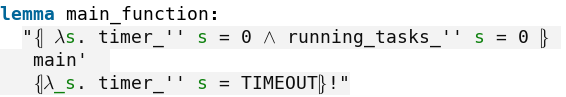
\includegraphics[width=0.45\textwidth]{main_lemma.png}}
\caption{Definition of invariant and measure for main loop} 
\label{fig}
\end{figure}
We can apply these two definitions via the \textit{whileLoop\_add\_inv} monad and obtain a proof goal that can be further broken into smaller goals using the weakest precondition tool.
\section{Conclusions}
The seL4 project has made outstanding contributions to the verification of C programs, offering a comprehensive set of proofs ranging from common security issues (integrity, confidentiality, availability) to detailed modeling of code behavior after compilation. These proofs were performed in order to obtain a kernel that could be used in real life scenarios. The importance of the project is augumented by the solutions implemented on the way to achieving this goal:
\begin{itemize}
    \item functional correctness proof of the seL4 microkernel;
    \item implementing proofs on the binary code;
    \item creation of a system through which the correspondence between the binary file and the source code from which it was compiled is verified;
    \item analysis of the C code and its automatic translation into a functional language on which reasoning can be built.
\end{itemize}
An encouraging conclusion of this project is that the automatic abstraction of the source code using the AutoCorres tool reduces the complexity of the effort to demonstrate \cite{sweat} the properties of the system. \\
This direction could facilitate the inclusion of verification as an important step in the development of software projects. With this idea in mind, we tried to include a kernel driver, but some other components of a kernel or general C programs could be verified if they meet the language subset limitations. These constraints seem to be the major barrier for expanding the C-to-Isabelle and AutoCorres tools into a generalized framework for safely translating C code into theorems. If the step of this translation could allow all programming language features to be used, some other C critical programs could be brought into Isabelle and reason about the correctness of their specifications.

\begin{thebibliography}{20}
\bibitem{greenaway} D. Greenaway, \textit{Automated proof-producing abstraction of C code},  Ph.D. Dissertation, School of Computer Science and Engineering, University of NSW, Sydney, Australia, August 2014, web source: https://ts.data61.csiro.au/publications/nicta\_full\_text/8758.pdf.
\bibitem{sweat}  D. Greenaway, J. Lim, J. Andronick, G. Klein, \textit{Don’t Sweat the Small Stuff - Formal Verification of C Code Without the Pain}, NICTA and UNSW, Sydney, Australia, web source: https://ts.data61.csiro.au/publications/nicta\_full\_text/7629.pdf.
\bibitem{sel4-wp} G. Heiser, \textit{The seL4 Microkernel - An Introduction}, White paper, The seL4 Foundation, Rev. 1.2, 2020.
\bibitem{verifos} G. Klein, J. Andronick, K. Elphinstone, T. Murray, T. Sewel, R. Kolanski, G. Heiser, NICTA and UNSW, \textit{Comprehensive Formal Verification of an OS Microkernel}, Sydney, Australia, ACM Transactions on Computer Systems, Vol. 32, No. 1, Art. 2, February 2014.
\bibitem{sel4} G. Klein, K. Elphinstone, G. Heiser, J. Andronick, D. Cock, P. Derrin, D. Elkaduwe, K. Engelhardt, R. Kolanski, M. Norrish, T. Sewell, H. Tuch, and S. Winwood, \textit{seL4: Formal Verification of an OS Kernel}, ACM Symposium on Operating Systems Principles, MT, USA, 2009.
\bibitem{tuch} H. Tuch, G. Klein, M. Norrish, \textit{Types, Bytes, and Separation Logic}, Proceedings of the 34th ACM SIGPLAN-SIGACT Symposium on Principles of Programming Languages, Nice, France, 97-108, 2007.
\bibitem{iso} International standard ISO/IECISO/IEC 9899, Committee Draft,  September 7, 2007, web source: http://www.open-std.org/jtc1/sc22/wg14/www/docs/n1256.pdf.
\bibitem{funcprog} R. Bird and P. Wadler, \textit{Introduction to Functional Programming}, Prentice Hall, Englewood Cliffs, 1988.
\bibitem{burstall} R. Burstall, \textit{Some techniques for proving correctness of programs which alter data structures}, Machine Intelligence 7, 1972.
\bibitem{isabelle1} T. Nipkov, \textit{Programming and Proving in Isabelle/HOL}, web source:  https://isabelle.in.tum.de/doc/prog-prove.pdf, checked on July 2021.
\bibitem{isabelle} Web source Isabelle homepage: https://isabelle.in.tum.de/.
\bibitem{pistachio} Web source L4Ka Pistachio: https://www.l4ka.org/65.php.
\bibitem{fiasco} Web source L4Re Fiasco: https://l4re.org/fiasco/build.html.
\bibitem{hazelnut} Web source L4Ka Hazelnut: https://github.com/l4ka/hazelnut. 
\bibitem{octrng} Web source: https://github.com/openbsd/src/blob/master/sys/arch/octeon/ dev/octrng.c.
\end{thebibliography}
\end{document}
